В данной главе описывается экспериментальная оценка прототипа распределенного MoE слоя на клиент-серверной архитектуре. Цель экспериментов состоит в том, чтобы сравнить производительность реализованного подхода с решениями, основанными на коллективных коммуникациях, а также проверить динамическую балансировку нагрузки и устойчивость системы к отказам экспертных блоков.

\subsection{Методика экспериментальной оценки}

\begin{table}[ht!]
    \centering
    \caption{Конфигурация экспериментального стенда}
    \label{tab:experiment-setup}
    \begin{tabularx}{\textwidth}{|>{\RaggedRight\arraybackslash}p{0.35\textwidth}|X|}
        \hline
        \textbf{Параметр} & \textbf{Значение} \\
        \hline
        GPU & 8$\times$ NVIDIA H100 \\
        \hline
        Объем видеопамяти & 80 GB \\
        \hline
        Связь между видеокартами & InfiniBand \\
        \hline
    \end{tabularx}
\end{table}

\subsection{Производительность MoE инференса}

В данном эксперименте измерялась производительность одного распределенного MoE слоя при передаче данных по RDMA с одним экспертным блоком~\cite{nvidiaGpudirectRdma}. Конфигурация слоя взята из архитектуры моделей семейства Qwen3 и включала 128 экспертов, top-\(k = 8\), размер скрытого состояния 2048, промежуточный размер экспертного блока 6144 и длину последовательности 200~\cite{qwen2025qwen3}. Для каждого размера батча выполнялось 16 прогревочных запусков и 32 запуска с измерением. Размер батча изменялся от 1000 до 9000 токенов с шагом 200 токенов.

Сравнивались четыре конфигурации реализации: базовая версия без дополнительных оптимизаций, версия с выравниванием экспертных активаций, версия с grouped GeMM и версия, в которой одновременно включены выравнивание и grouped GeMM. Измерения проводились отдельно для двух движков передачи данных: NIXL и MoonCake Transfer Engine~\cite{nvidiaNixl,mooncakeTransferEngine}. Также на графиках задержки приведен ориентир на коллективную реализацию DeepEP~\cite{deepseekDeepEP}.

На графиках представлены два типа измерений. Первый соответствует случайной инициализации весов роутера, при которой входной поток распределяется между практически всеми экспертами. Второй соответствует весам роутера из модели Qwen3-30B-A3B; в этом случае активируется небольшая часть экспертов, порядка 10\% от их общего числа~\cite{qwen2025qwen3}.

Для графиков задержки дополнительно показан разброс измерений: нижняя и верхняя границы области соответствуют 1-му и 99-му перцентилям.

\begin{figure}[ht!]
    \centering
    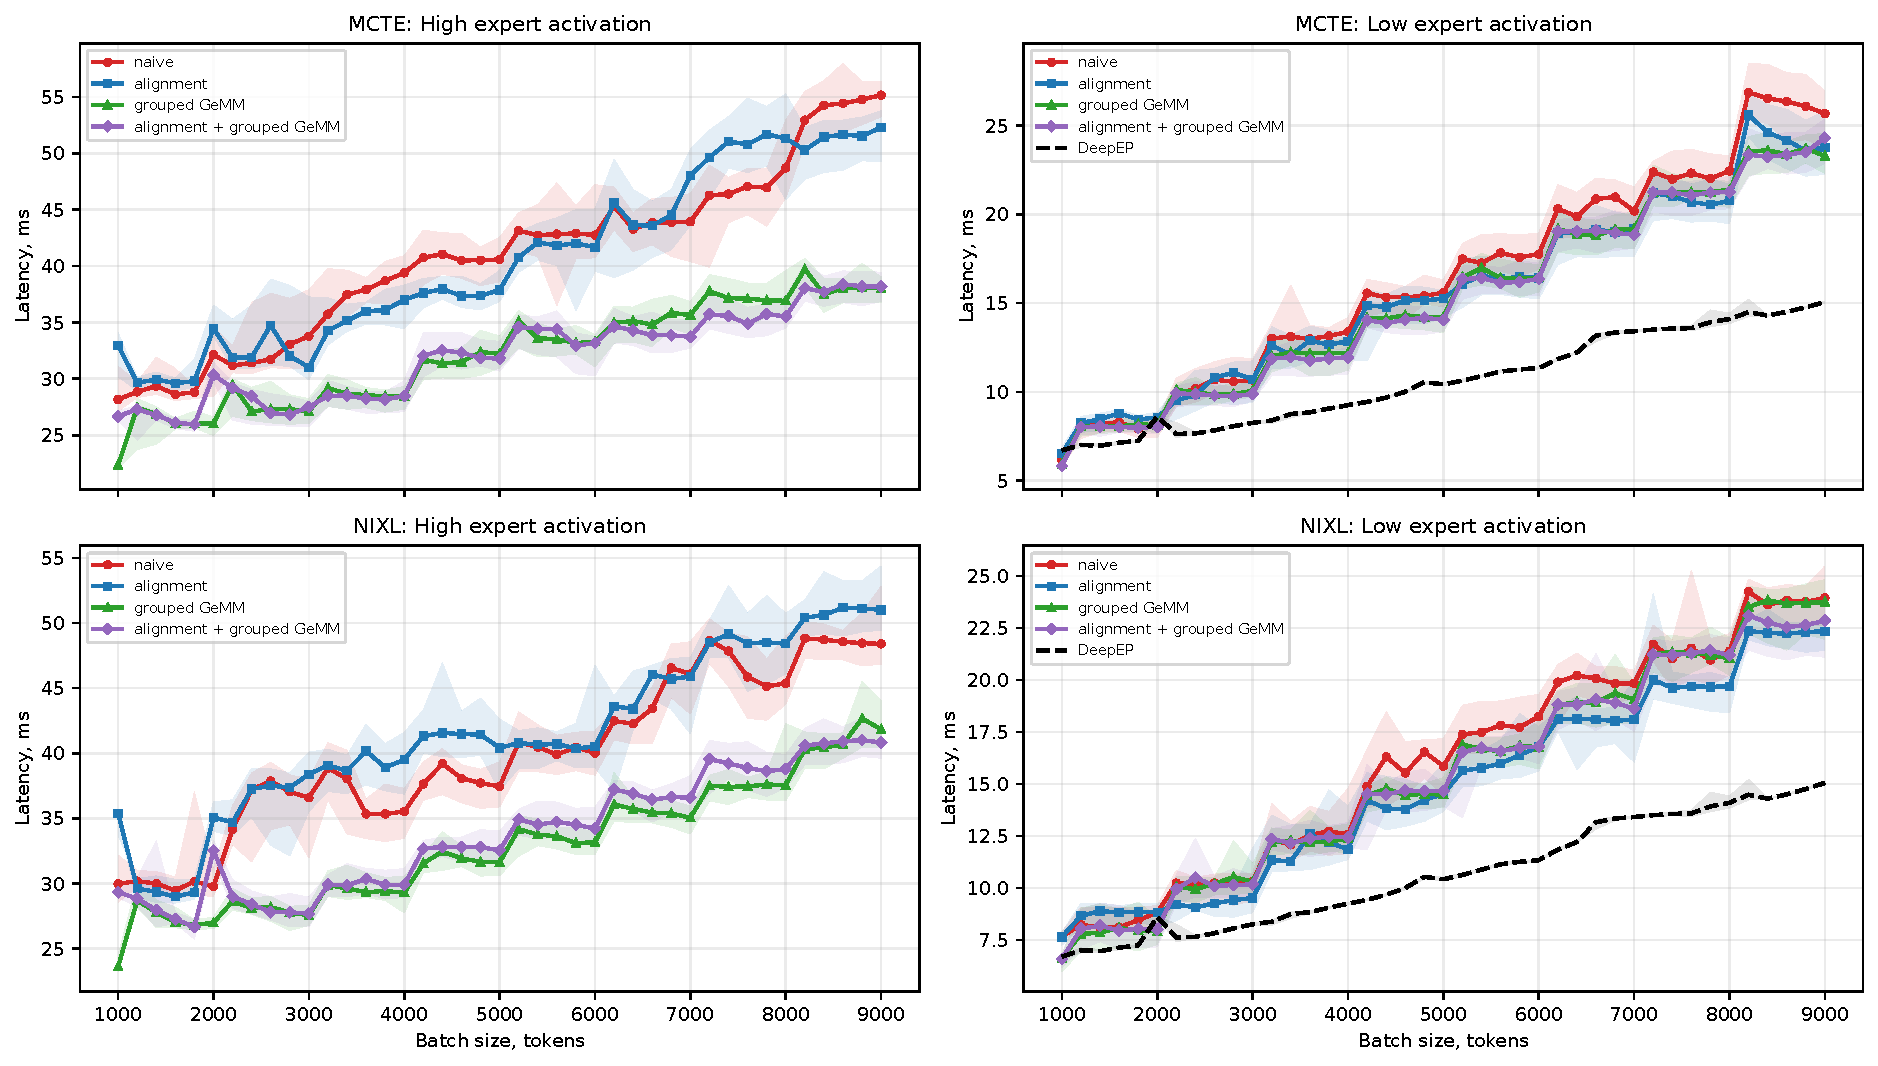
\includegraphics[width=\textwidth]{diagrams/experiments/latency_comparison.pdf}
    \caption{Сравнение задержки MoE слоя при использовании RDMA}
    \label{fig:moe-latency-comparison}
\end{figure}

Рисунок~\ref{fig:moe-latency-comparison} показывает, что grouped GeMM наиболее заметно снижает задержку в сценарии с большим числом активных экспертов. В этом режиме на каждого эксперта приходится меньше активаций, поэтому буфер, обрабатываемый экспертным блоком, разбивается на большое число небольших фрагментов. Последовательное выполнение отдельных матричных умножений в такой ситуации увеличивает накладные расходы, тогда как grouped GeMM позволяет объединить несколько экспертных вычислений в одну более крупную GPU-операцию. В сценарии с малым числом активных экспертов абсолютная задержка ниже, а различия между конфигурациями менее выражены, поскольку каждый эксперт обрабатывает более крупные фрагменты буфера.

\begin{figure}[ht!]
    \centering
    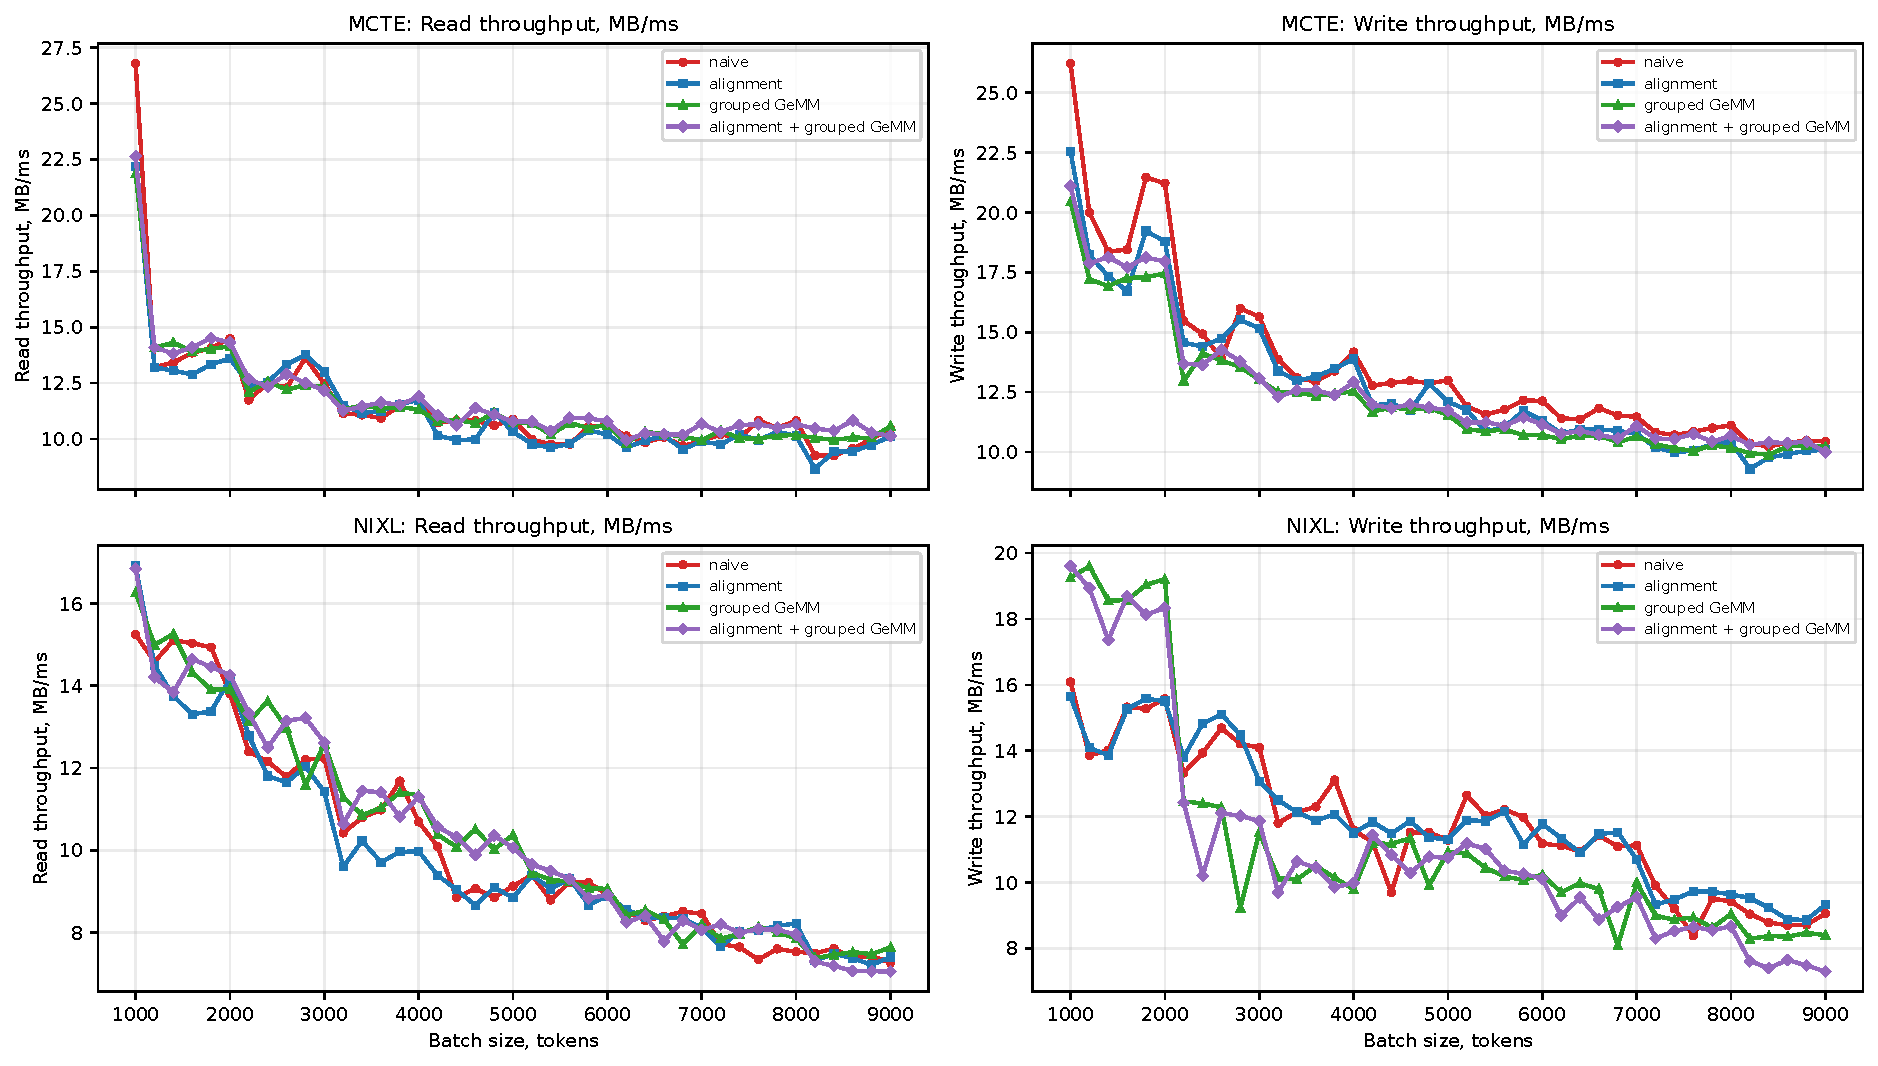
\includegraphics[width=\textwidth]{diagrams/experiments/throughput_analysis.pdf}
    \caption{Пропускная способность чтения и записи при передаче данных MoE слоя по RDMA}
    \label{fig:moe-throughput-analysis}
\end{figure}

На рисунке~\ref{fig:moe-throughput-analysis} приведена средняя пропускная способность операций переноса памяти для сценария с малым числом активных экспертов. По мере увеличения размера батча пропускная способность отдельной операции чтения или записи снижается. Это связано с тем, что в асинхронном рантайме одновременно выполняется больше конкурентных операций переноса памяти, а общая пропускная способность шины ограничена. Поэтому средняя скорость отдельного переноса уменьшается, но при этом растет совокупная загрузка канала передачи данных.

\begin{figure}[ht!]
    \centering
    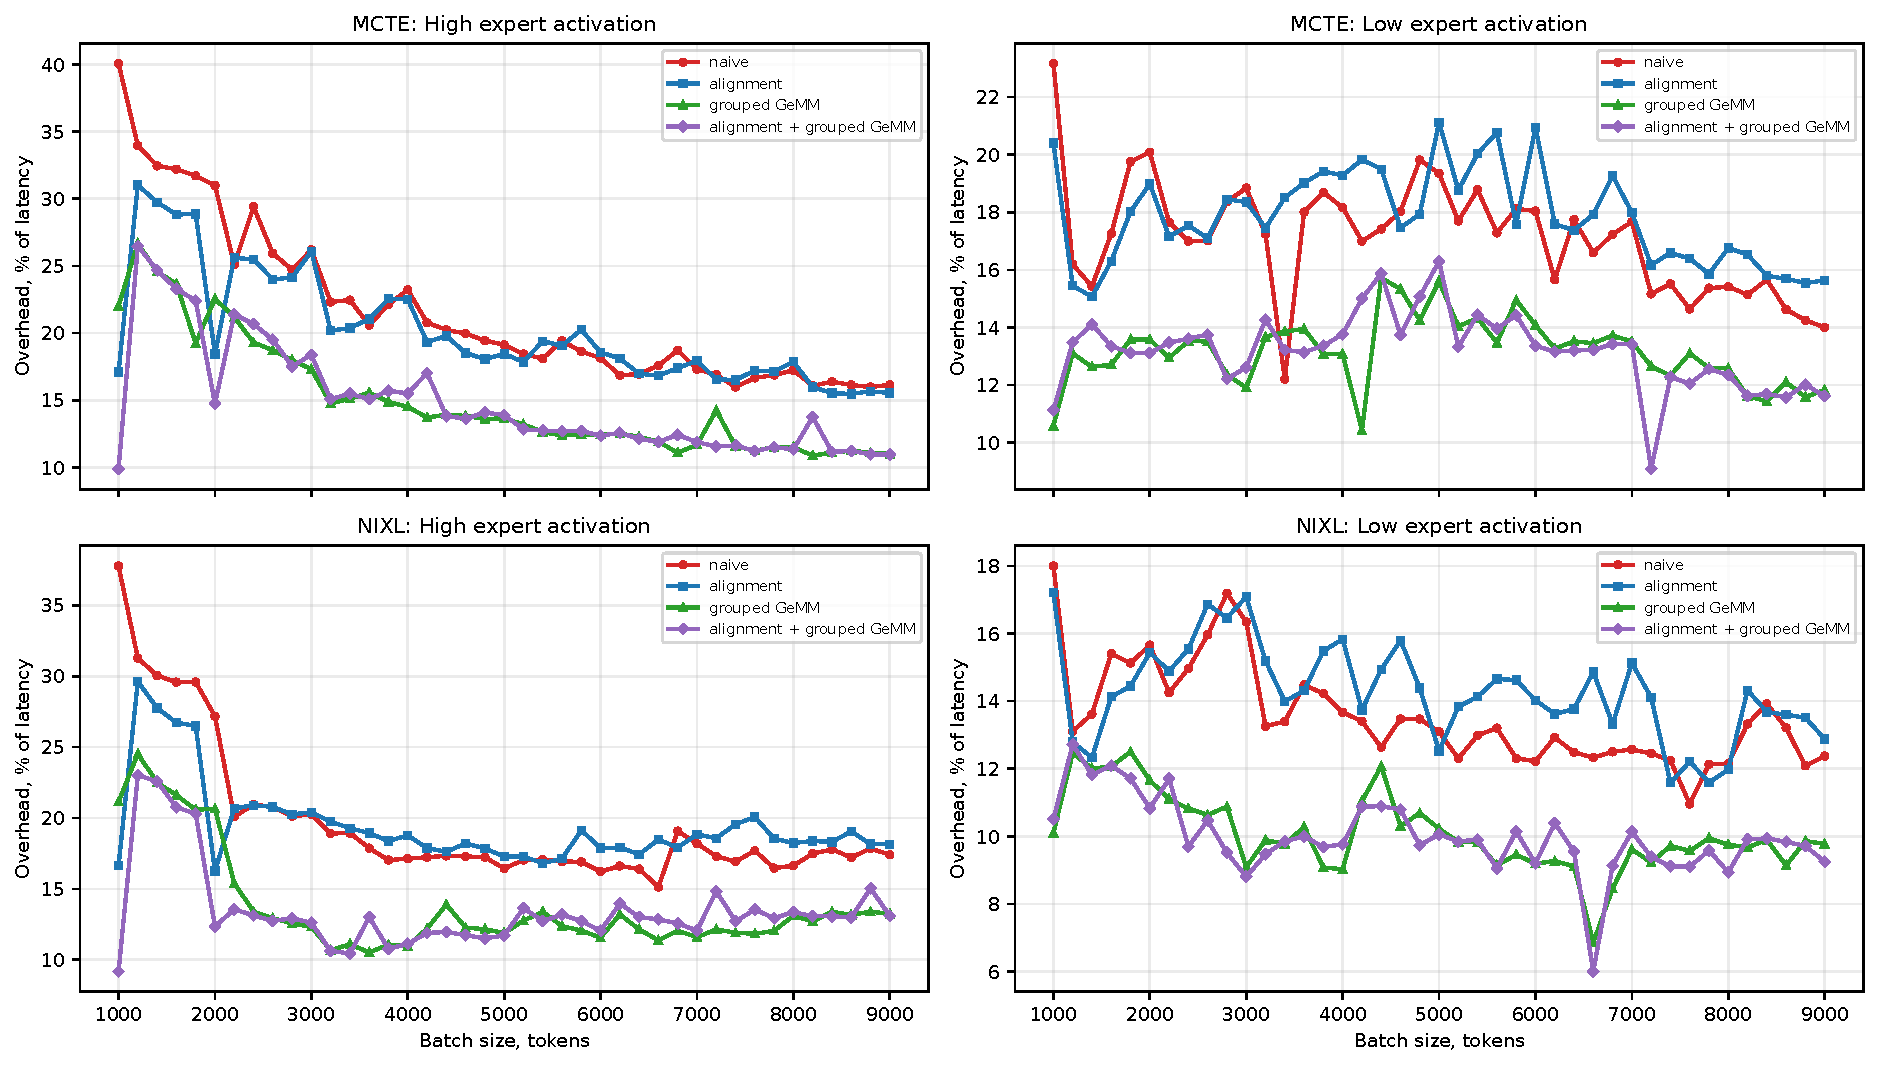
\includegraphics[width=\textwidth]{diagrams/experiments/overhead_analysis.pdf}
    \caption{Доля накладных расходов в задержке MoE слоя при использовании RDMA}
    \label{fig:moe-overhead-analysis}
\end{figure}

На рисунке~\ref{fig:moe-overhead-analysis} приведена средняя доля накладных расходов в общей задержке слоя. Эта величина вычисляется как разность между временем выполнения всей задачи на экспертном блоке и суммарным временем экспертных вычислений, чтения и записи данных.
Результаты показывают, что более сильное дробление буфера приводит к росту доли накладных расходов. При этом с увеличением размера батча эта доля растет умеренно, что указывает на сохранение устойчивого поведения системы при росте нагрузки.

\subsection{Балансировка нагрузки и отказоустойчивость}

Для проверки устойчивости к частичным отказам был проведен эксперимент с фиксированной целевой нагрузкой 50 запросов в секунду. В предлагаемой архитектуре использовались два экспертных блока, размещенные на разных GPU; в коллективной реализации использовались два ранга. В момент времени \(t_1\), отмеченный красной вертикальной линией, один экспертный блок исключался из пула доступных исполнителей. После этого система должна была продолжить обработку запросов на оставшемся экспертном блоке. В момент времени \(t_2\), отмеченный зеленой вертикальной линией, в пул добавлялся новый экспертный блок с той же конфигурацией гиперпараметров, после чего ожидалось восстановление пропускной способности до уровня, близкого к исходному. Для коллективной реализации аналогичный сценарий моделировался отказом одного ранга: после такого отказа следующий вызов dispatch или combine на оставшемся ранге приводит к ошибке, поскольку коллективная операция больше не может быть выполнена всей заданной группой участников.

\begin{figure}[ht!]
    \centering
    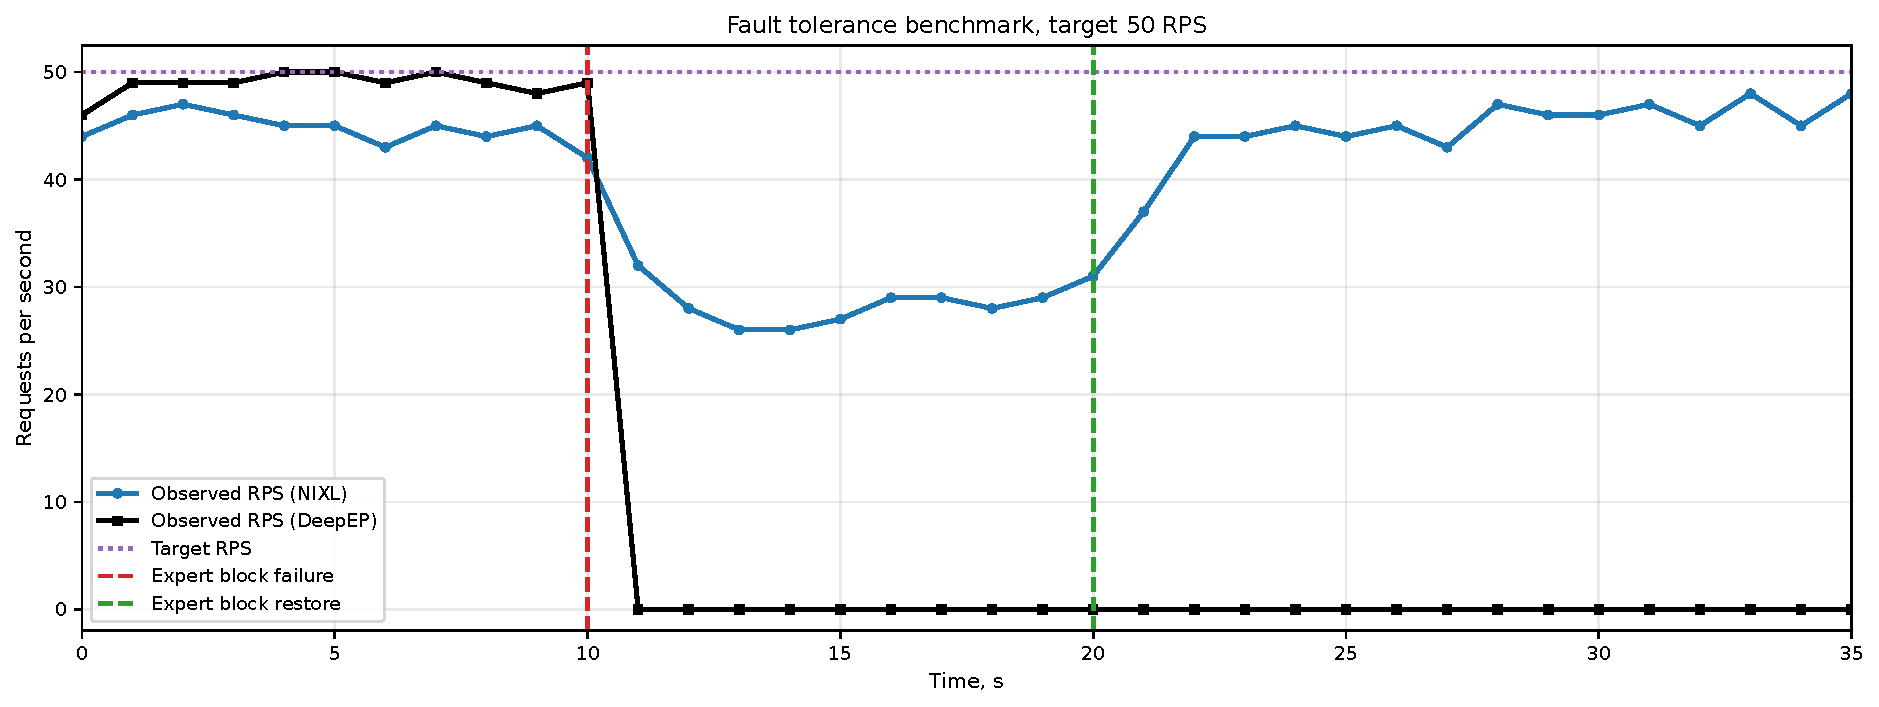
\includegraphics[width=\textwidth]{diagrams/experiments/fault_tolerance_rps_timeline_rps_50.pdf}
    \caption{Изменение пропускной способности при временном отказе экспертного блока}
    \label{fig:fault-tolerance-rps-timeline}
\end{figure}

На рисунке~\ref{fig:fault-tolerance-rps-timeline} показана динамика пропускной способности во времени для предлагаемой реализации и коллективной реализации DeepEP~\cite{deepseekDeepEP}. После отказа одного из двух экспертных блоков наблюдается снижение пропускной способности, однако обработка запросов не прекращается. Такое поведение соответствует цели предлагаемой архитектуры: продолжать инференс на оставшихся доступных эспертных блоках, даже при отказе одного или нескольких из них.

Для DeepEP в данном эксперименте отказ одного ранга приводит к падению пропускной способности до нуля: коллективная операция требует участия всей группы участников, поэтому отказ даже одного из них приводик к падению всей системы.

После добавления нового экспертного блока пропускная способность предлагаемой реализации возвращается к уровню, близкому к целевой нагрузке. Таким образом, эксперимент показывает практическую пользу динамического управления пулом исполнителей: система деградирует контролируемо, а не останавливает инференс целиком.

\subsection*{Выводы по главе}
\addcontentsline{toc}{subsection}{Выводы по главе}

В главе оцениваются основные свойства предлогаемой архитектуры инфренеса MoE слоя: производительность, накладные расходы на клиент-серверную природу инференса, поведение при изменении нагрузки, возможность динамической балансировки нагрузки и отказоустойчивость.

Ожидаемый итог экспериментальной части состоит в следующем: предложенный подход уступает высоко оптимизированным коллективным решениям по пиковой производительности, но обеспечивает динамическую балансировку нагрузки и сохранение работоспособности при частичных отказах клиентских узлов.
